\section{Сухое электронно-лучевое травление резиста}

Как было отмечено, в существующих методах микро- и нано-структурирования, основанных на термической деполимеризации резиста, нагревание резиста носит локальный характер -- как по времени, так и в пространстве. В отличие от них в методе термостимулированной электронно-лучевой литографии резист остается полностью прогретым на протяжении всего процесса экспонирования. За счет этого метод обеспечивает производительность, в десятки раз превышающую таковую в классической электронно-лучевой литографии. Помимо этого, глобальный характер нагрева резиста приводит к тому, что важным фактором, определяющим форму профиля в резисте, становятся процессы оплавления резиста. Здесь наблюдается определенное сходство с вышеописанным методом полутоновой литографии, которая часто включает в себя стадию оплавления резиста для сглаживания границ различных участков. Однако, в методе термостимулированной электронно-лучевой литографии оплавление не является отдельной стадией, а происходит одновременно со всеми остальными процессами, такими как электронно-стимулированная деполимеризация резиста и диффузия мономера. Именно одновременное протекание всех процессов, определяющий форму линии в данном методе, делает его сложным для теоретического исследования. До настоящего времени метод исследовался в большей степени экспериментально, и далее будут подробно описаны шаги, предшествовавшие настоящей работе.


\subsection{Цепная термическая деполимеризация полимеров}
В первых работах по изучению термической деполимеризации проводилось облучение виниловых полимеров ультрафиолетом при температурах выше их температуры стеклования (120--200 $^\circ$C)~\cite{Cowley_1952_1, Cowley_1952_2, Grassie1949_1, Grassie1949_2, Grassie1949_3, Grassie1949_4}. Анализ молекулярно-массового распределения облученных полимеров, получаемого методом гель-проникающей хроматографии, и продуктов распада позволил сделать вывод о цепном характере реакции деполимеризации полимера и получить оценку длины цепи деполимеризации. Были установлены процессы, протекающие при термической деполимеризации полимеров -- образование активного центра деполимеризации (инициирование кинетической цепи деполимеризации), его распространение вдоль молекулы (рост кинетической цепи) и возможный перенос на другую молекулу, а также исчезновение активного центра деполимеризации за счет различных эффектов. Были предложены кинетические уравнения, связывающие данные процессы с результатами эксперимента, что позволило оценить значения констант данных процессов.

На рисунке~\ref{fig:Cowley_Mn} приведены зависимости отношения среднечисловой молекулярной массы облученного полимера ($M_n$) к исходной среднечисловой молекулярной массе ($M_{n0}$) от степени деградации полимера. Как видно, для образцов высоким значением $M_{n0}$ отношение $M_n / M_{n0}$ уменьшается практически линейно, в то время как для образцов с более низким значением $M_{n0}$ данное отношение на начальных этапах деградации практически не изменяется. Для обоснования этого явления было выдвинуто предположение о том, что реакция деполимеризации носит цепной характер. Длина цепи деполимеризации при этом такова, что длинные молекулы распадаются не до конца, что приводит к изменению $M_n$. В то же время относительно короткие (относительно длины цепи деполимеризации) молекулы распадаются полностью, что исключает их вклад в $M_n$.

\begin{figure}
	\centering
	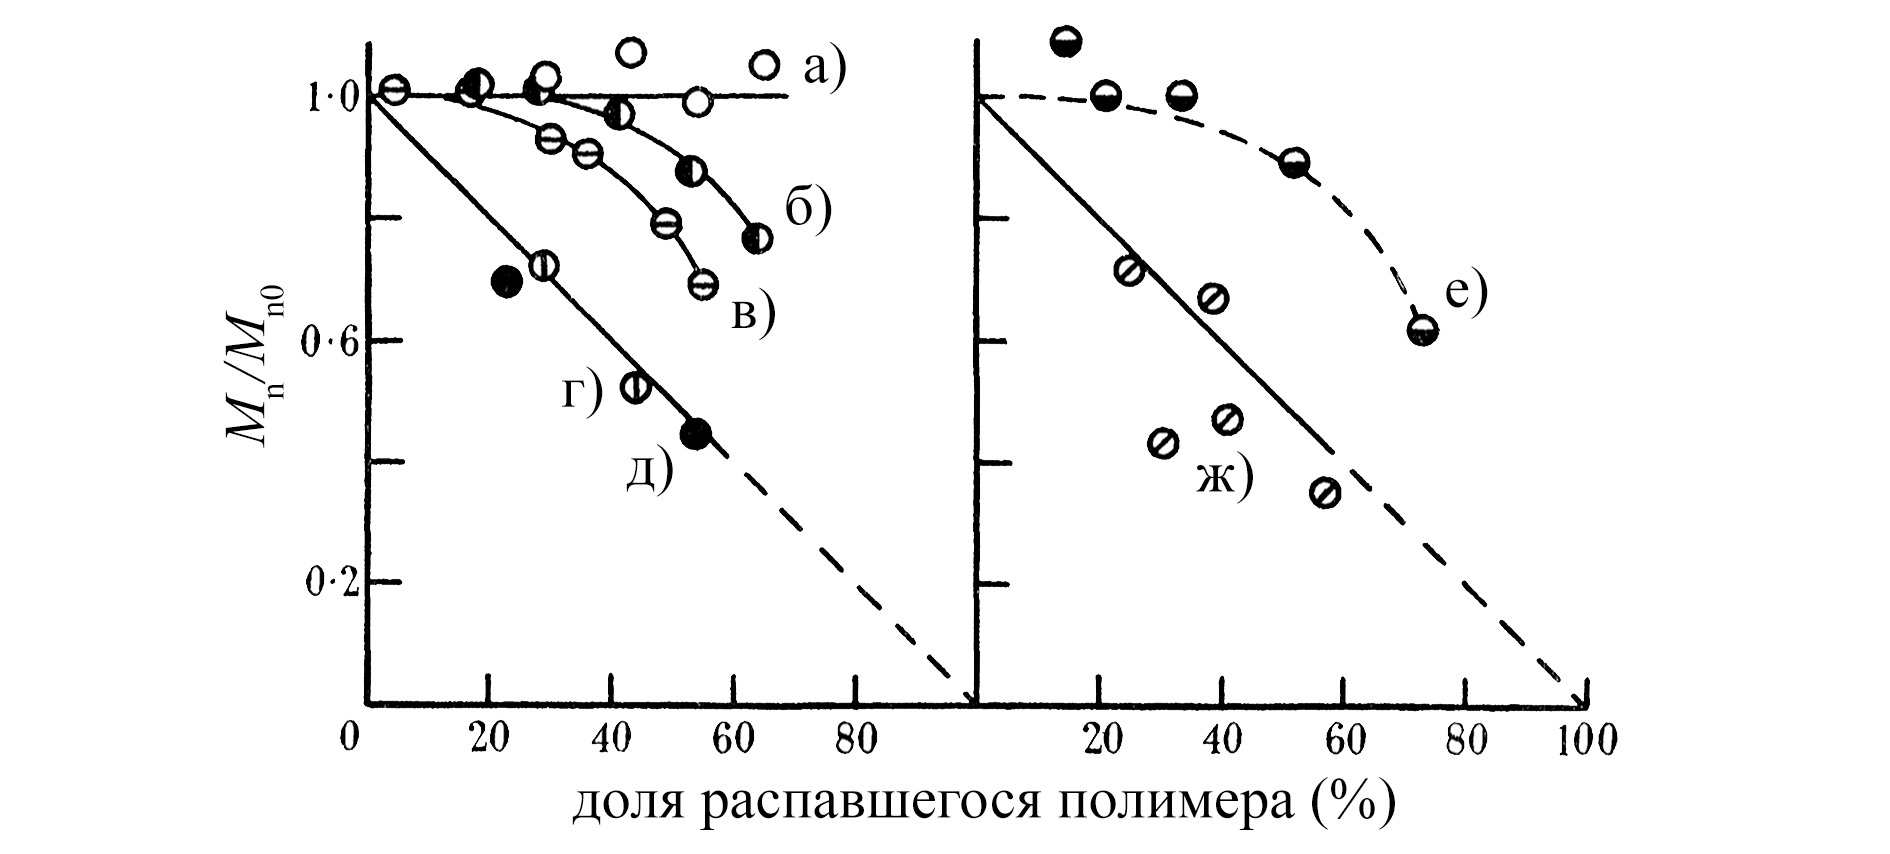
\includegraphics{jpg/Cowley_Mn_14pt}
	\caption{Зависимость отношения $M_n / M_{n0}$ от доли распавшегося полимера при термической (а)-д)) и фотоинициированной (е)-ж)) деполимеризации ПММА для различных значений $M_{n0}$: a) 44300, б) 94000, в) 179000, г) 650000, д) 725000, е) 125000, ж) 770000~\cite{Cowley_1952_1}.}
	\label{fig:Cowley_Mn}
\end{figure}

Последующие исследования на основе Фурье-спектроскопии позволили более детально описать процесс термической деполимеризации. Так, например, анализ интенсивности отдельных полос спектра, соответствующим различным связям в полимерной молекуле, позволил определить основные механизмы радиационной деполимеризации~\cite{Bermudez} (см. рисунок~\ref{fig:PMMA_degpaths}). В дальнейшем, наиболее полная картина процессов термической деполимеризации была сформирована уже за счет применения методов молекулярной динамики~\cite{Stoliarov}.

\begin{figure}
	\centering
	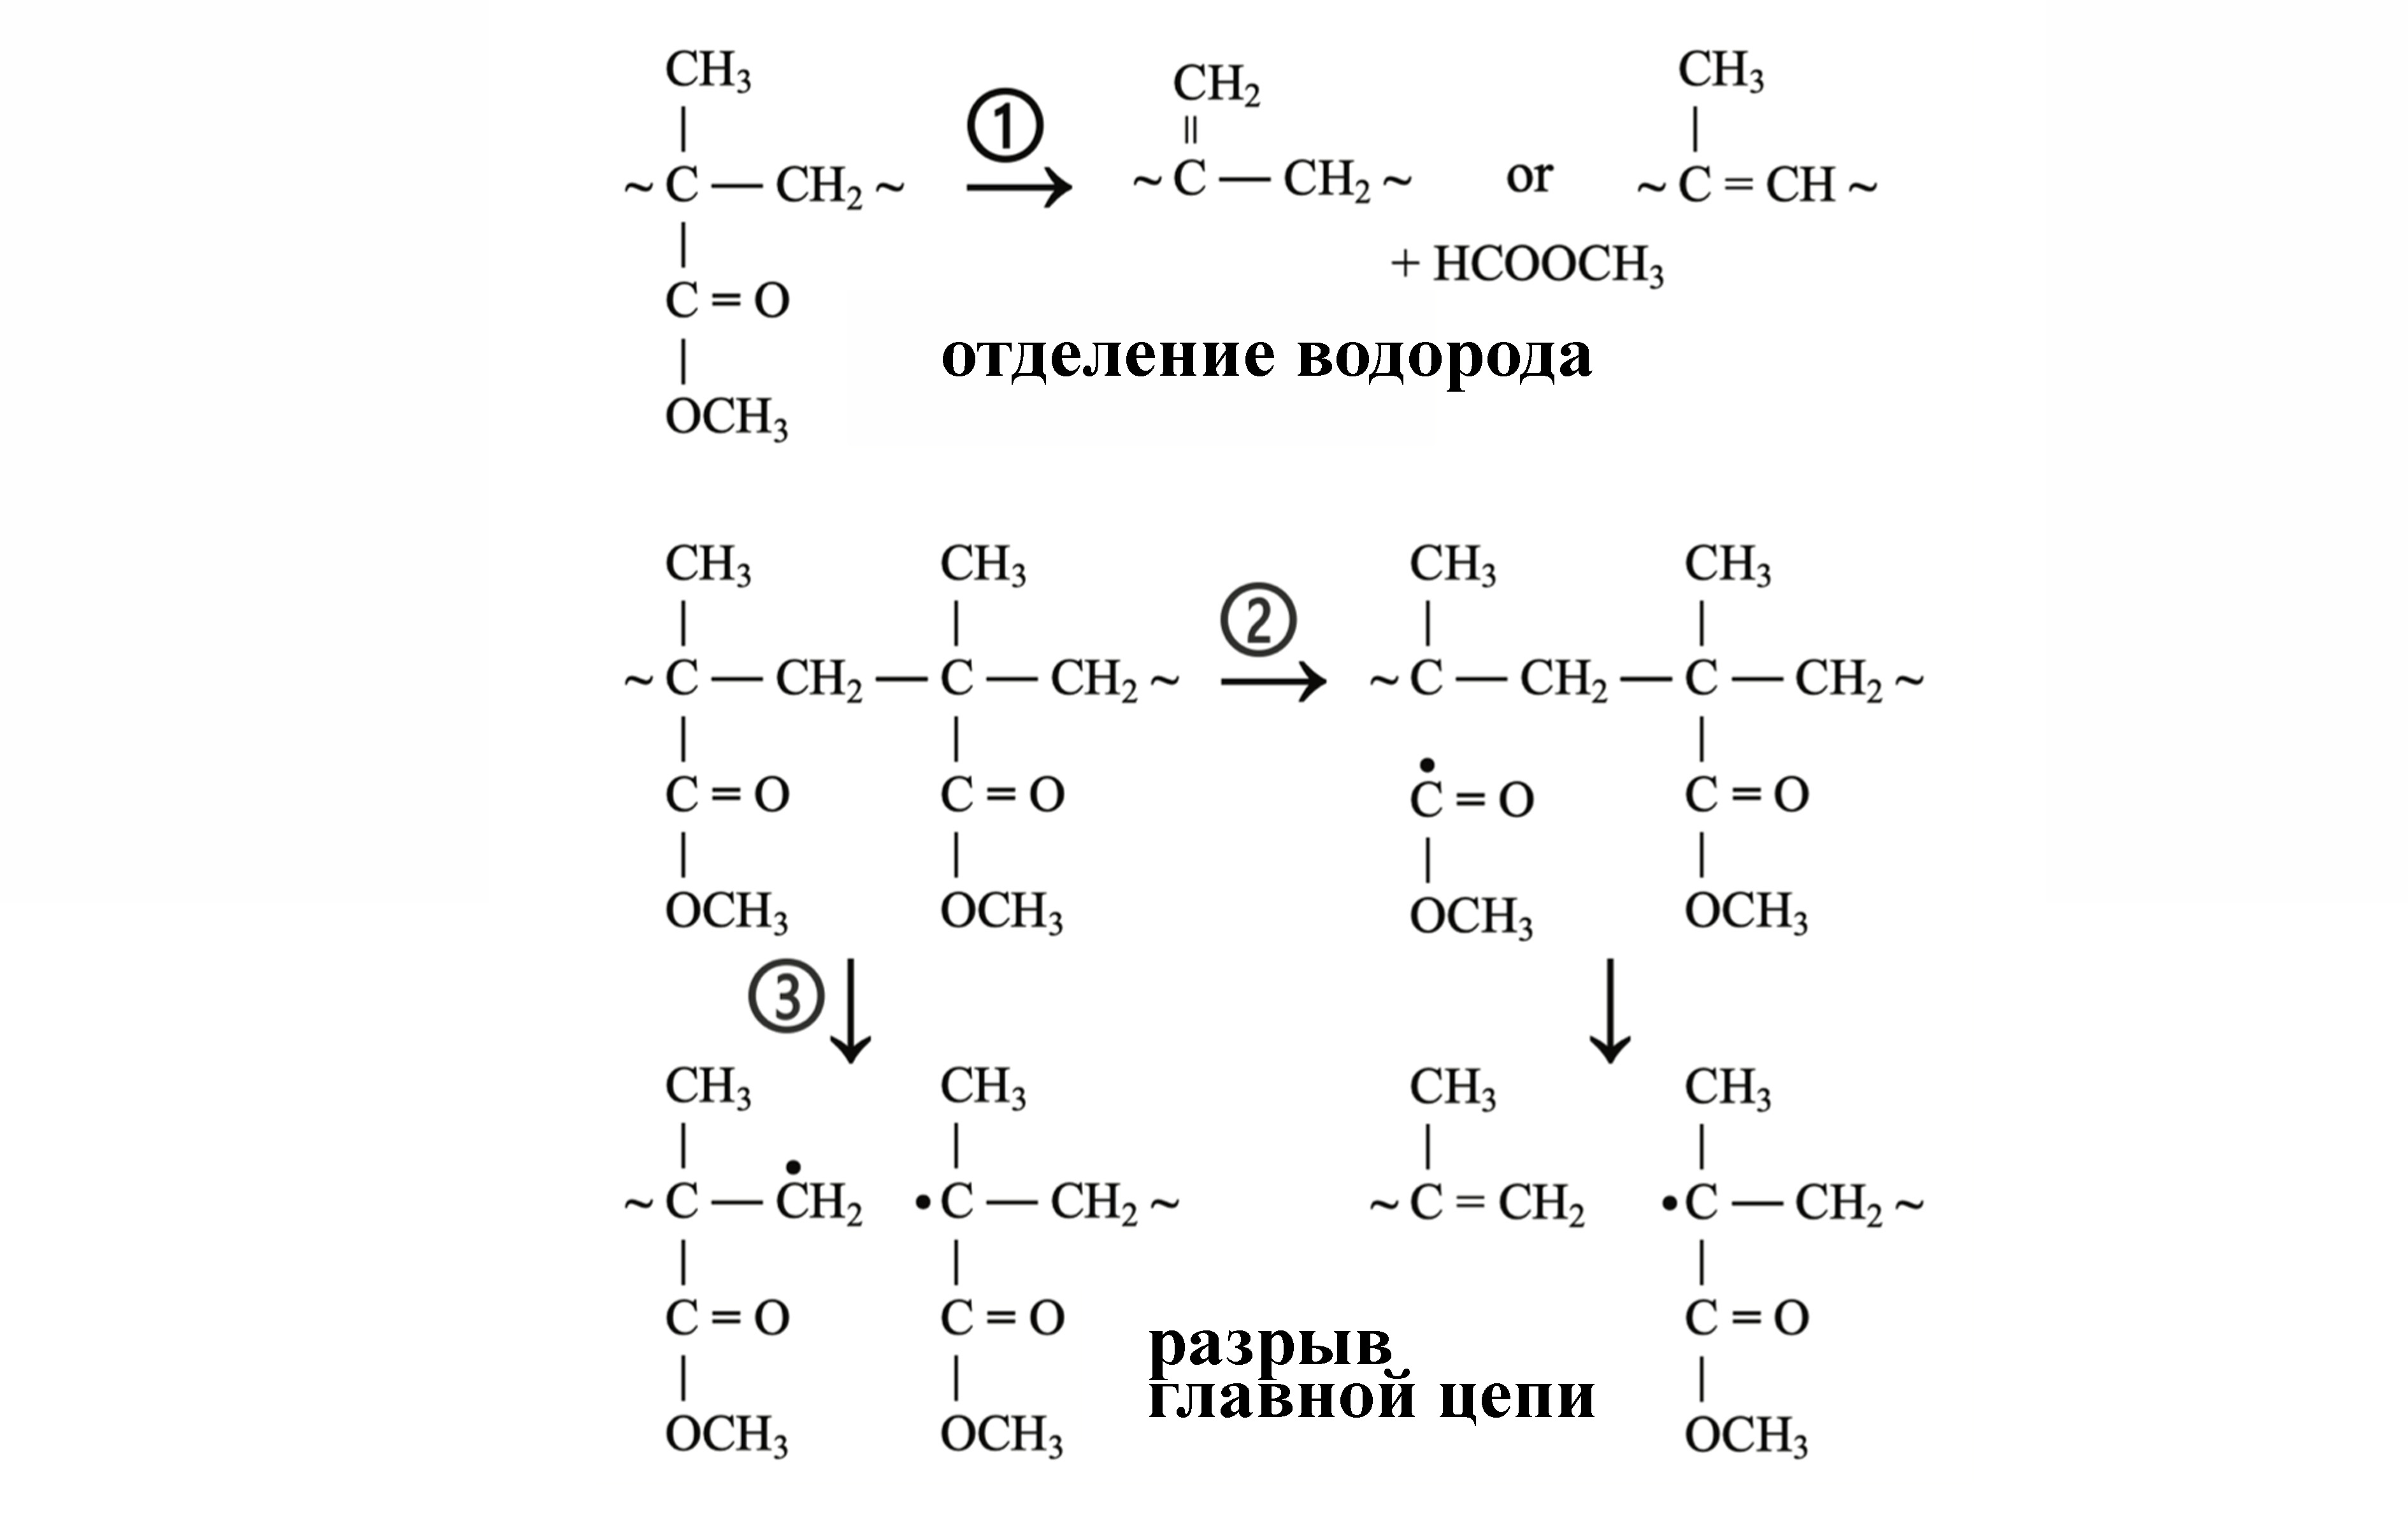
\includegraphics{jpg/PMMA_degpaths_14pt}
	\caption{Схематическое изображение основных реакций, протекающих в ПММА под действием внешнего излучения~\cite{Bermudez}.}
	\label{fig:PMMA_degpaths}
\end{figure}

Важной характерной особенностью процесса термической деполимеризации является тот факт, что энергия активации процесса термического образования активного центра деполимеризации превышает энергию активации процесса его распространения вдоль полимерной молекулы~\cite{Cowley_1952_1, Sanchez-Jimenez_Ea}. Это означает, что существует область температур, в которой цепная реакция деполимеризации может протекать только при условии, что активный центр деполимеризации был образован по механизму, отличному от термического. Таким механизмом может являться локальное воздействие внешнего излучения, что приводит к концепции метода микролитографии на основе термической деполимеризации, инициируемой локально.

Первое упоминание о возможном применении термической деполимеризации резиста в микро- и наноструктурировании встречается в работе, посвященной ионностимулированной термической деполимеризации полиметилметакрилата (ПММА)~\cite{Fragala_1}. В последующих работах этого автора была изложена подробная модель образования и выхода мономера из слоя полимера (ПММА) при ионностимулированной термической деполимеризации~\cite{Fragala_2,Fragala_3_diffusion}, \linebreak однако, к идее микролитографии на основе данного метода он уже не возвращается.


\subsection{Развитие метода микролитографии на основе термической деполимеризации резиста}
Первые шаги в изучении метода микролитографии на основе термической деполимеризации резиста описываются в работе~\cite{Bruk_2000}. В ней приводятся результаты инициированной $\gamma$-излучением деполимеризации ПММА в виде нанометрового слоя, адсорбированного на поверхности пор силохрома. Несмотря на то, что в данной работе термическая деполимеризация не использовалась для формирования структуры в резисте, а исследовалась в общем, результаты работы позволили определить особенности потенциально возможного метода микроструктурирования на основе этого явления. Так, например, были получены оценки для времени диффузии мономера в слое ПММА после разрушения молекулы и длины кинетической цепи деполимеризации, сделаны выводы о масштабах протекания процессов передачи активного центра деполимеризации на мономер и полимер. Также было установлено, что при термической деполимеризации ПММА при температурах 120-180 $^\circ$C влияние процессов реполимеризации пренебрежимо мало.

Впоследствии были проведены эксперименты по изучению термической деполимеризации полиметилметакрилата (ПММА), протекающей при экспонировании электронным лучом, а также впервые были продемонстрированы двумерные и трехмерные структуры, полученные в ПММА в этом процессе~\cite{Bruk_2013}. Такой метод формирования получил название СЭЛТР -- сухое электронно-лучевое травление резиста. Методика экспериментов была следующей:
\begin{enumerate}
	\item На пластину монокристаллического кремния методом \textquotedbl spin-coating\textquotedbl{} из 2\%-ного раствора в анизоле с последующей сушкой наносили слой ПММА-резиста марки 950К толщиной $L_0$ = 80-85 нм;
	\item Полученные образцы помещали на специальный нагреватель, вводили в камеру электронного микроскопа Camscan или Ultra-55, разогревали до нужной температуры и в вакууме порядка 10$^{-5}$ мбар подвергали экспонированию электронным лучом в режиме сканирования вдоль линии либо по заданной площади;
	\item После экспонирования нагревательный элемент отключался, и резист остывал в камере электронного микроскопа в вакууме естественным образом; время остывания в зависимости от начальной температуры резиста составляло приблизительно 100-200 с;
	\item Толщину слоя резиста до и после травления, а также форму получаемых пространственных фигур травления определяли методом атомно-силовой микроскопии на атомно-силовом микроскопе марки Solver P47-SPM-MTD.
\end{enumerate}

Энергия электронного пучка ($E$), ток при экспонировании ($I$) и диаметр сечения электронного луча ($\delta$) составляли примерно 20 кэВ, 1 нА и 200 нм, соответственно, для электронного микроскопа Camscan и 15 кэВ, 1.5 пА и 10 нм, соответственно, для электронного микроскопа Ultra-55.

Одним из важных результатов работы стали кинетические кривые травления в методе СЭЛТР -- зависимости нормализованной толщины слоя резиста $L_{\text{норм}} = L/L_0$ ($L$ -- толщина слоя резиста в данный момент времени) от дозы экспонирования (рисунок~\ref{fig:kin_curves}). Было установлено, что доза полутравления $D_{0.5}$ (доза, необходимая для травления слоя толщиной, равной половине начальной) составляет приблизительно 2.5 мкКл/см$^2$, 0.8 мкКл/см$^2$ и \linebreak 0.3 мкКл/см$^2$ для температур 125 $^\circ$С, 150 $^\circ$С и 170 $^\circ$C, соответственно. Дозы полного травления слоя резиста $D_1$ для этих же температур составили приблизительно 20, 12 и 6.5 мкКл/см$^2$. Таким образом, дозы $D_1$ приблизительно в 10 раз (а дозы полутравления приблизительно в 100 раз) меньше доз $D_1$ и $D_{0.5}$, необходимых при формировании позитивной маски или рельефа в ПММА-резисте в стандартной электронно-лучевой литографии по \textquotedbl мокрой\textquotedbl{} технологии (для которой $D_1$ составляет примерно 100 мкКл/см$^2$).

\begin{figure}
	\centering
	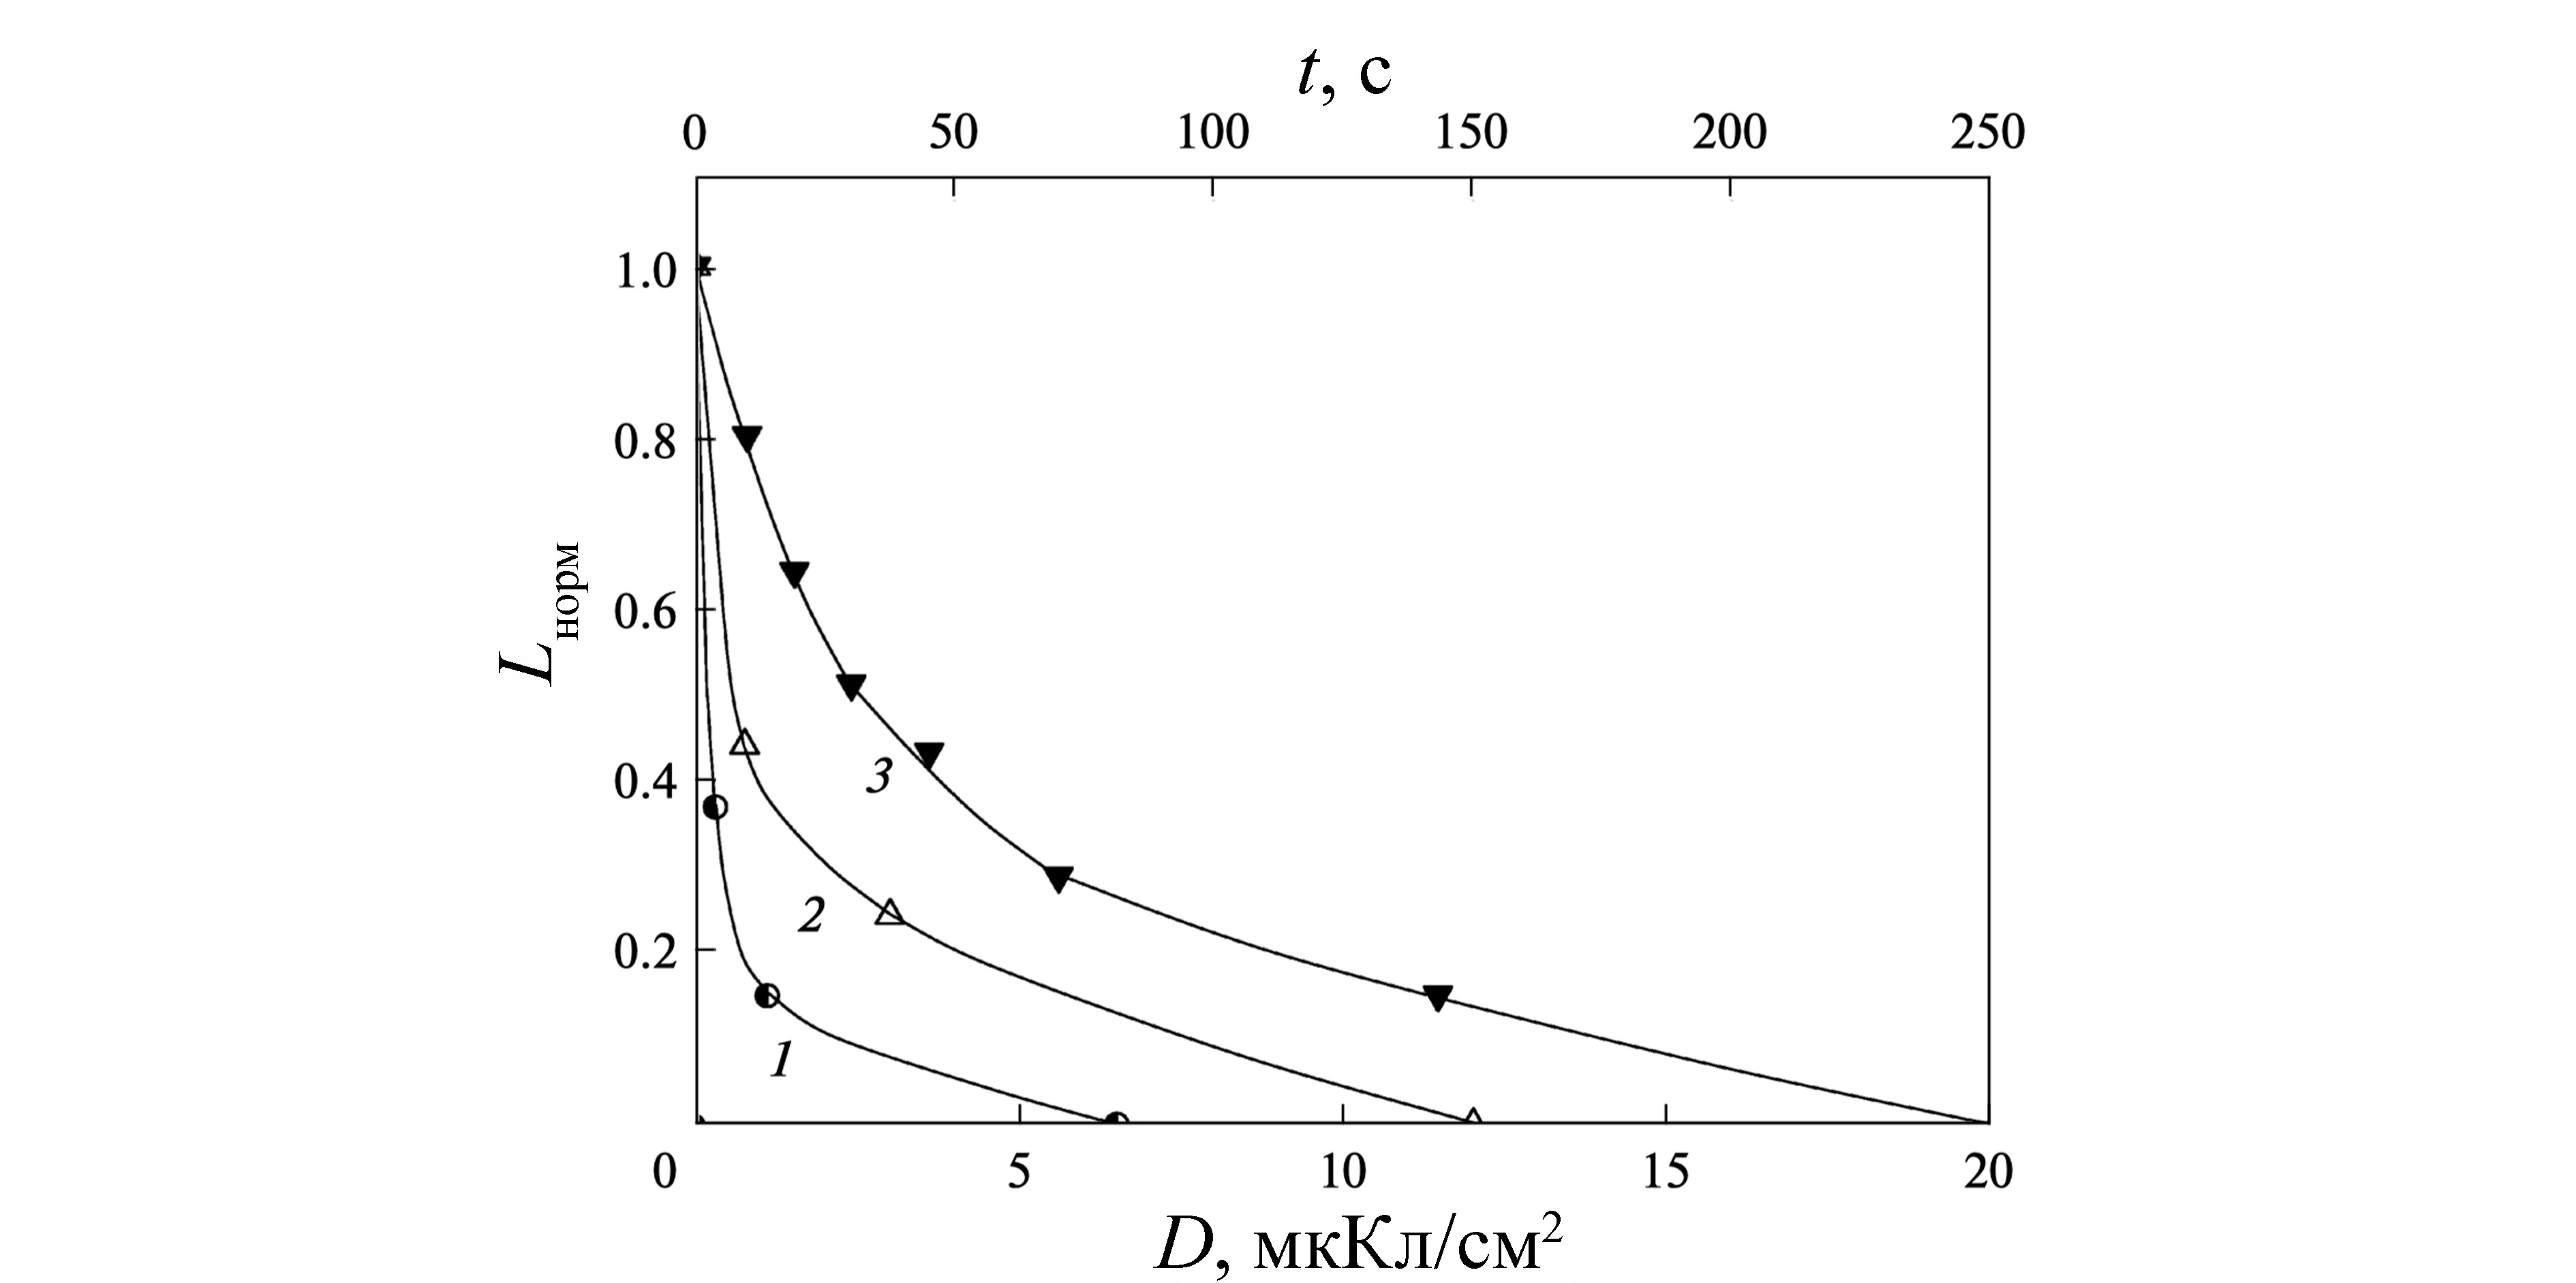
\includegraphics{jpg/DEBER_kin_curves_14pt}
	\caption{Кинетические кривые травления ПММА в методе СЭЛТР, полученные для температур 125 $^\circ$С (1), 150 $^\circ$С (2) и 170 $^\circ$С (3)~\cite{Bruk_2013}.}
	\label{fig:kin_curves}
\end{figure}

Было сделано предположение, что в условиях проведенных опытов процесс травления протекал одновременно по всей толщине слоя резиста, а формирование рельефа обусловлено объемной релаксацией полимера, которая протекает достаточно быстро по сравнению с временем эксперимента. Более того, считалось, что скорость процесса травления приблизительно одинакова по всей толщине слоя резиста, соответственно, она пропорциональна текущей толщине слоя и уменьшается по ходу процесса по мере уменьшения этой толщины. Это утверждение предполагает, что в проведенных опытах происходила эффективная диффузия образующихся молекул мономера из слоя резиста по всей его толщине, так что процесс диффузии мономера в газовую фазу не лимитировал скорость травления. Для обоснования этих предположений была введена приведенная скорость травления $W_{\text{пр}}$ -- отношение средней скорости травления в некоторой точке кинетической кривой ($V_i$) к соответствующей этой точке толщине слоя резиста ($L_i$):
\begin{equation}
	W_{пр} = V_i / L_i
\end{equation}

На рисунке~\ref{fig:DEBER_W} приведена зависимость $W_{\text{пр}}$ от текущей нормированной толщины слоя резиста по ходу процесса травления при 125°C. Характер этой зависимости показывает, что даже в начале травления, когда толщина слоя максимальна, диффузия мономера из пленки протекает достаточно быстро по всей глубине экспонированной области и не влияет на общую скорость травления. Если бы скорость диффузии мономера тормозила процесс травления, то $W_{\text{пр}}$ должна была возрастать по ходу процесса, сопровождающемуся уменьшением текущей толщины слоя, поскольку, как известно, время диффузионного проскока молекул газа $\tau_{\text{диф}}$ пропорционально квадрату толщины слоя $l$, через который происходит диффузия~\cite{Bruk_2000}:
\begin{equation}
	\tau_{\text{диф}} = l^2 / 12 D,
\end{equation}
где $D$ -- эффективный коэффициент диффузии газа.

\begin{figure}
	\centering
	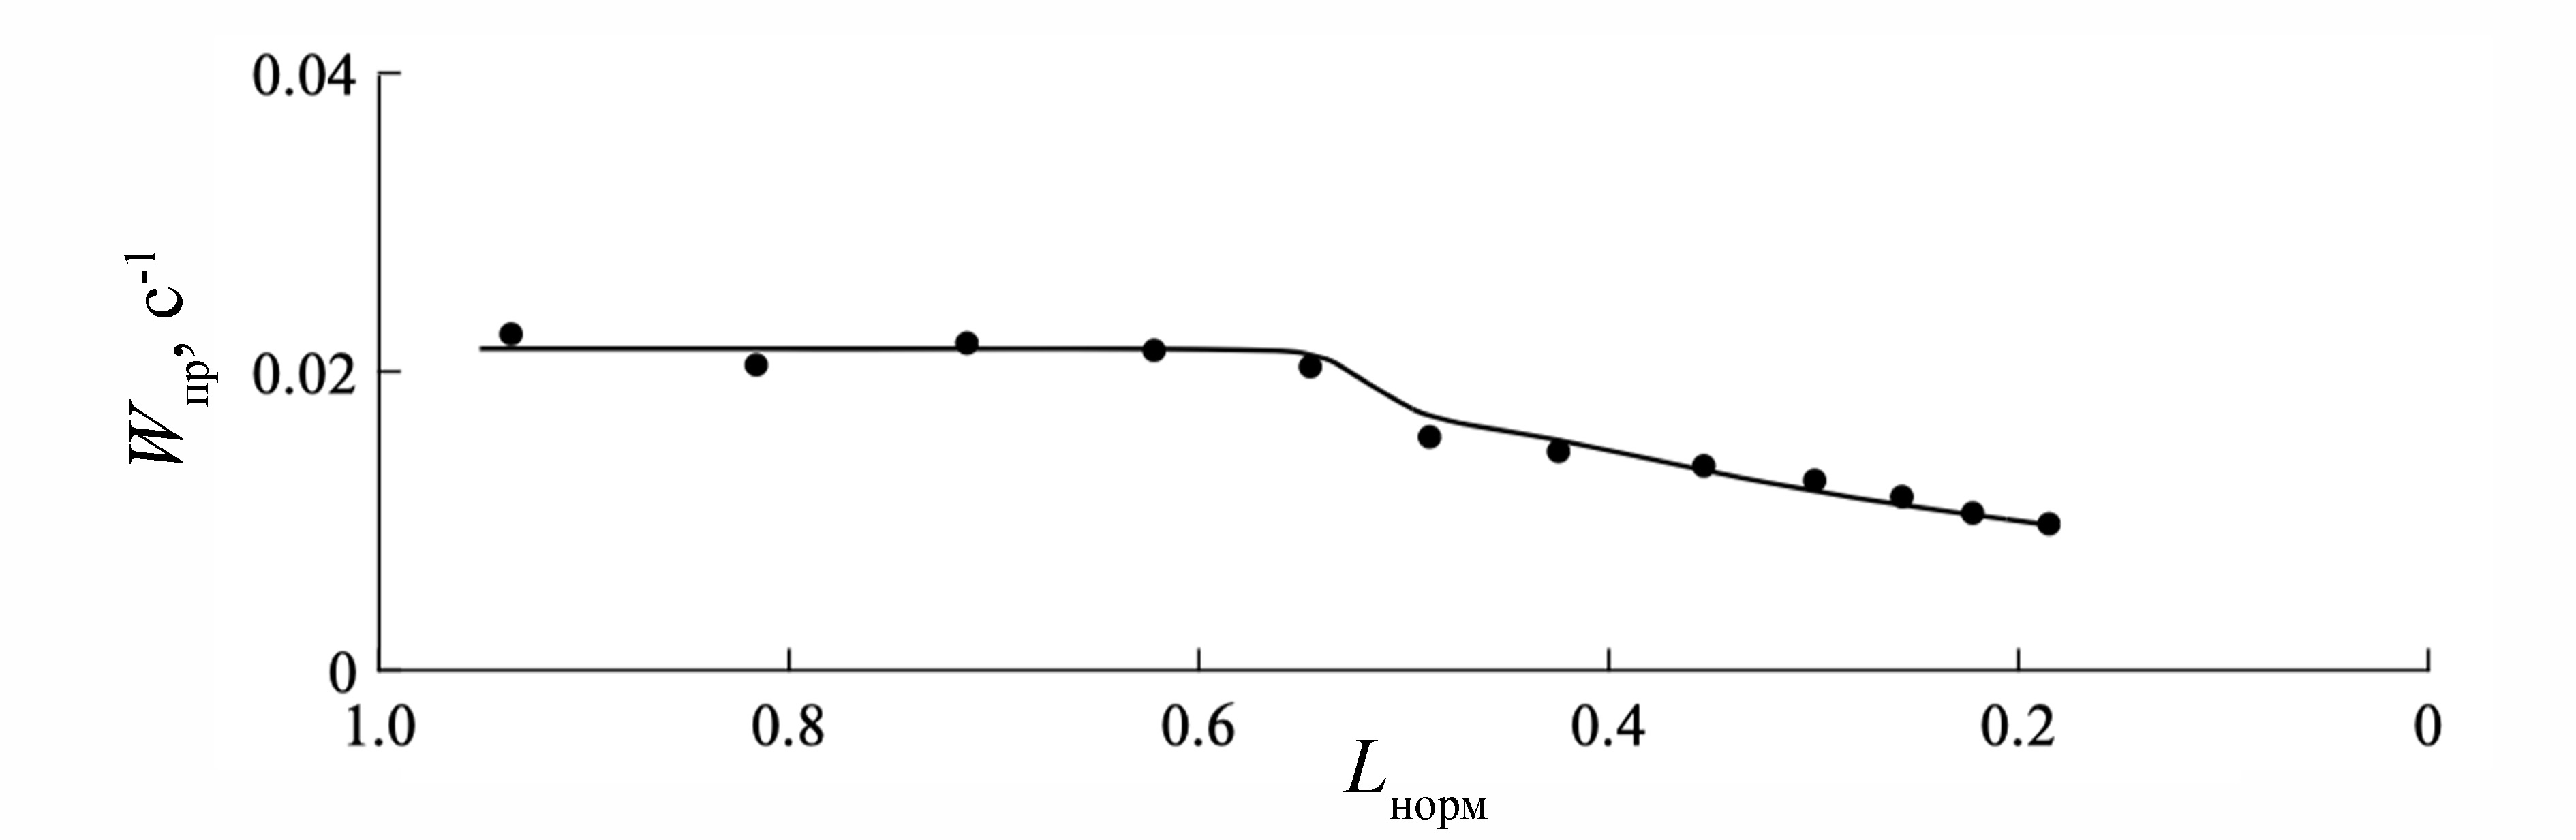
\includegraphics{jpg/DEBER_W_14pt}
	\caption{Зависимость приведенной скорости травления $W_{пр}$ для ПММА в методе СЭЛТР при температуре 125 $^\circ$C~\cite{Bruk_2013}.}
	\label{fig:DEBER_W}
\end{figure}

Из рисунка~\ref{fig:DEBER_W} видно, что возрастания скорости по ходу процесса не наблюдается -- вплоть до конверсий около 50\% приведенная скорость постоянна, после чего немного уменьшается. Наблюдаемое уменьшение $W_{\text{пр}}$ можно связать с уменьшением молекулярной массы полимера и(или) с возникновением в полимере по мере облучения дополнительных дефектов, ускоряющих обрыв кинетических цепей деполимеризации.

Также в работе~\cite{Bruk_2013} были проведены первые опыты по формированию методом СЭЛТР трехмерных ступенчатых структур -- на пластине с резистом, разогретой до необходимой температуры, при неизменном положении луча и пластины проводили последовательно несколько экспонирований при сканировании по различным последовательно уменьшающимся площадям (рисунок~\ref{fig:DEBER_stairs}). Первое экспонирование проводили на площади 100$\times$100 мкм, второе -- на площади 98$\times$98 мкм, третье -- на площади 96$\times$96 мкм и т. д. Соотношение линейных размеров площадей сканирования определяло ширину ступеней формирующихся на краю экспонированной площади. Дозы облучения для каждого экспонирования рассчитывались в соответствии с кинетической кривой травления, при этом для каждого последующего экспонирования учитывалась доза, полученная экспонируемой областью при предыдущем облучении. При этом была отмечена достаточно высокая однородность травления по оси $Z$: шероховатость ступенек шириной 5–10 мкм по оси Z составляла всего около 1–2 нм (в отличие от традиционной \textquotedbl мокрой\textquotedbl{} 3D литографии, при которой шероховатость по оси $Z$ обычно составляет 5–7 нм~\cite{Murali_e_beam_roughness}).
Была также отмечена невысокая контрастность получаемого изображения -- угол наклона стенок профиля относительно горизонтали составлял около 3$^\circ$. Было предположено, что основной причиной которой является специфическая форма кинетической кривой травления метода СЭЛТР, а также пониженная вязкость ПММА в условиях процесса СЭЛТР, приводящая к растеканию профиля.

\begin{figure}
	\centering
	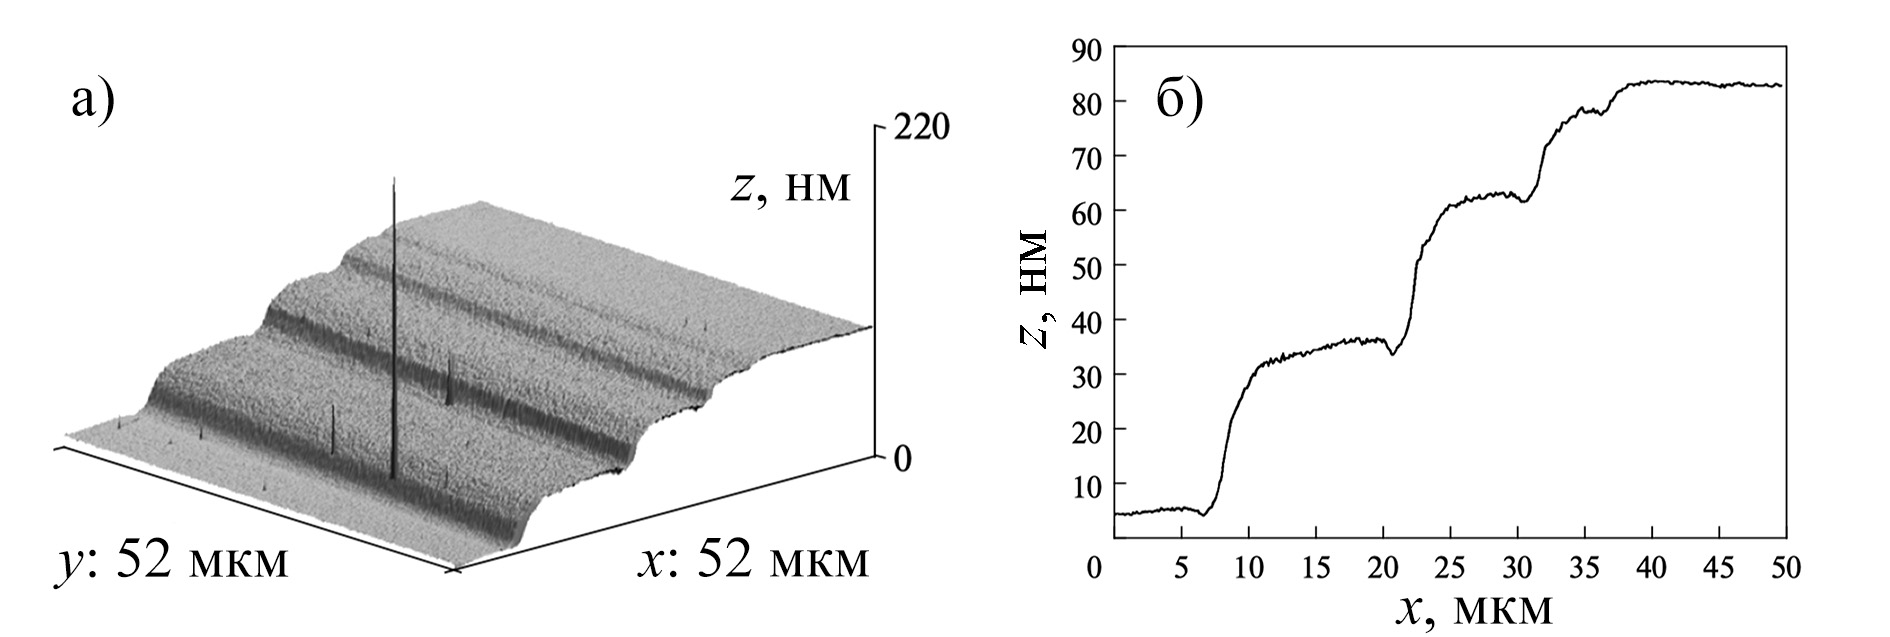
\includegraphics{jpg/DEBER_stairs_14pt}
	\caption{Ступенчатые профили, полученные в ПММА методом СЭЛТР при температуре 125 $^\circ$C~\cite{Bruk_2013}.}
	\label{fig:DEBER_stairs}
\end{figure}


\subsection{Текущая стадия разработки метода сухого электронно-лучевого травления резиста}

Наиболее актуальные на сегодняшний день экспериментальные результаты по исследованию метода сухого электронно-лучевого травления резиста приведены в работах~\cite{Bruk_2015_co, Bruk_2016_mee}. Помимо вышеописанных ступенчатых профилей, в этих работах исследовались периодические профили, полученные при экспонировании резиста электронным лучом вдоль серии параллельных линий (рисунок~\ref{fig:DEBER_many_profiles}). Было продемонстрировано, что при таком экспонировании результирующий профиль приобретает практически синусоидальную форму, что является аргументом в пользу применения метода СЭЛТР для формирования некоторых дифракционных оптических элементов~\cite{Mitreska_sin_gratings}. При этом снова была отмечена высокая производительность метода -- при температуре 160 $^\circ$C полное травление в центре линии было достигнуто при дозе экспонирования менее 1 мкКл/см$^2$. Также была продемонстрирована возможность достаточно точного переноса профиля, полученного в ПММА, на поверхность вольфрама и кремния за счет сухого травления в реакторе индуктивно-связанной плазмы (рисунок~\ref{fig:DEBER_Si_W}). Этот факт теоретически позволяет использовать метод СЭЛТР для формирования, например, штампов для термической НИЛ.

\begin{figure}
	\centering
	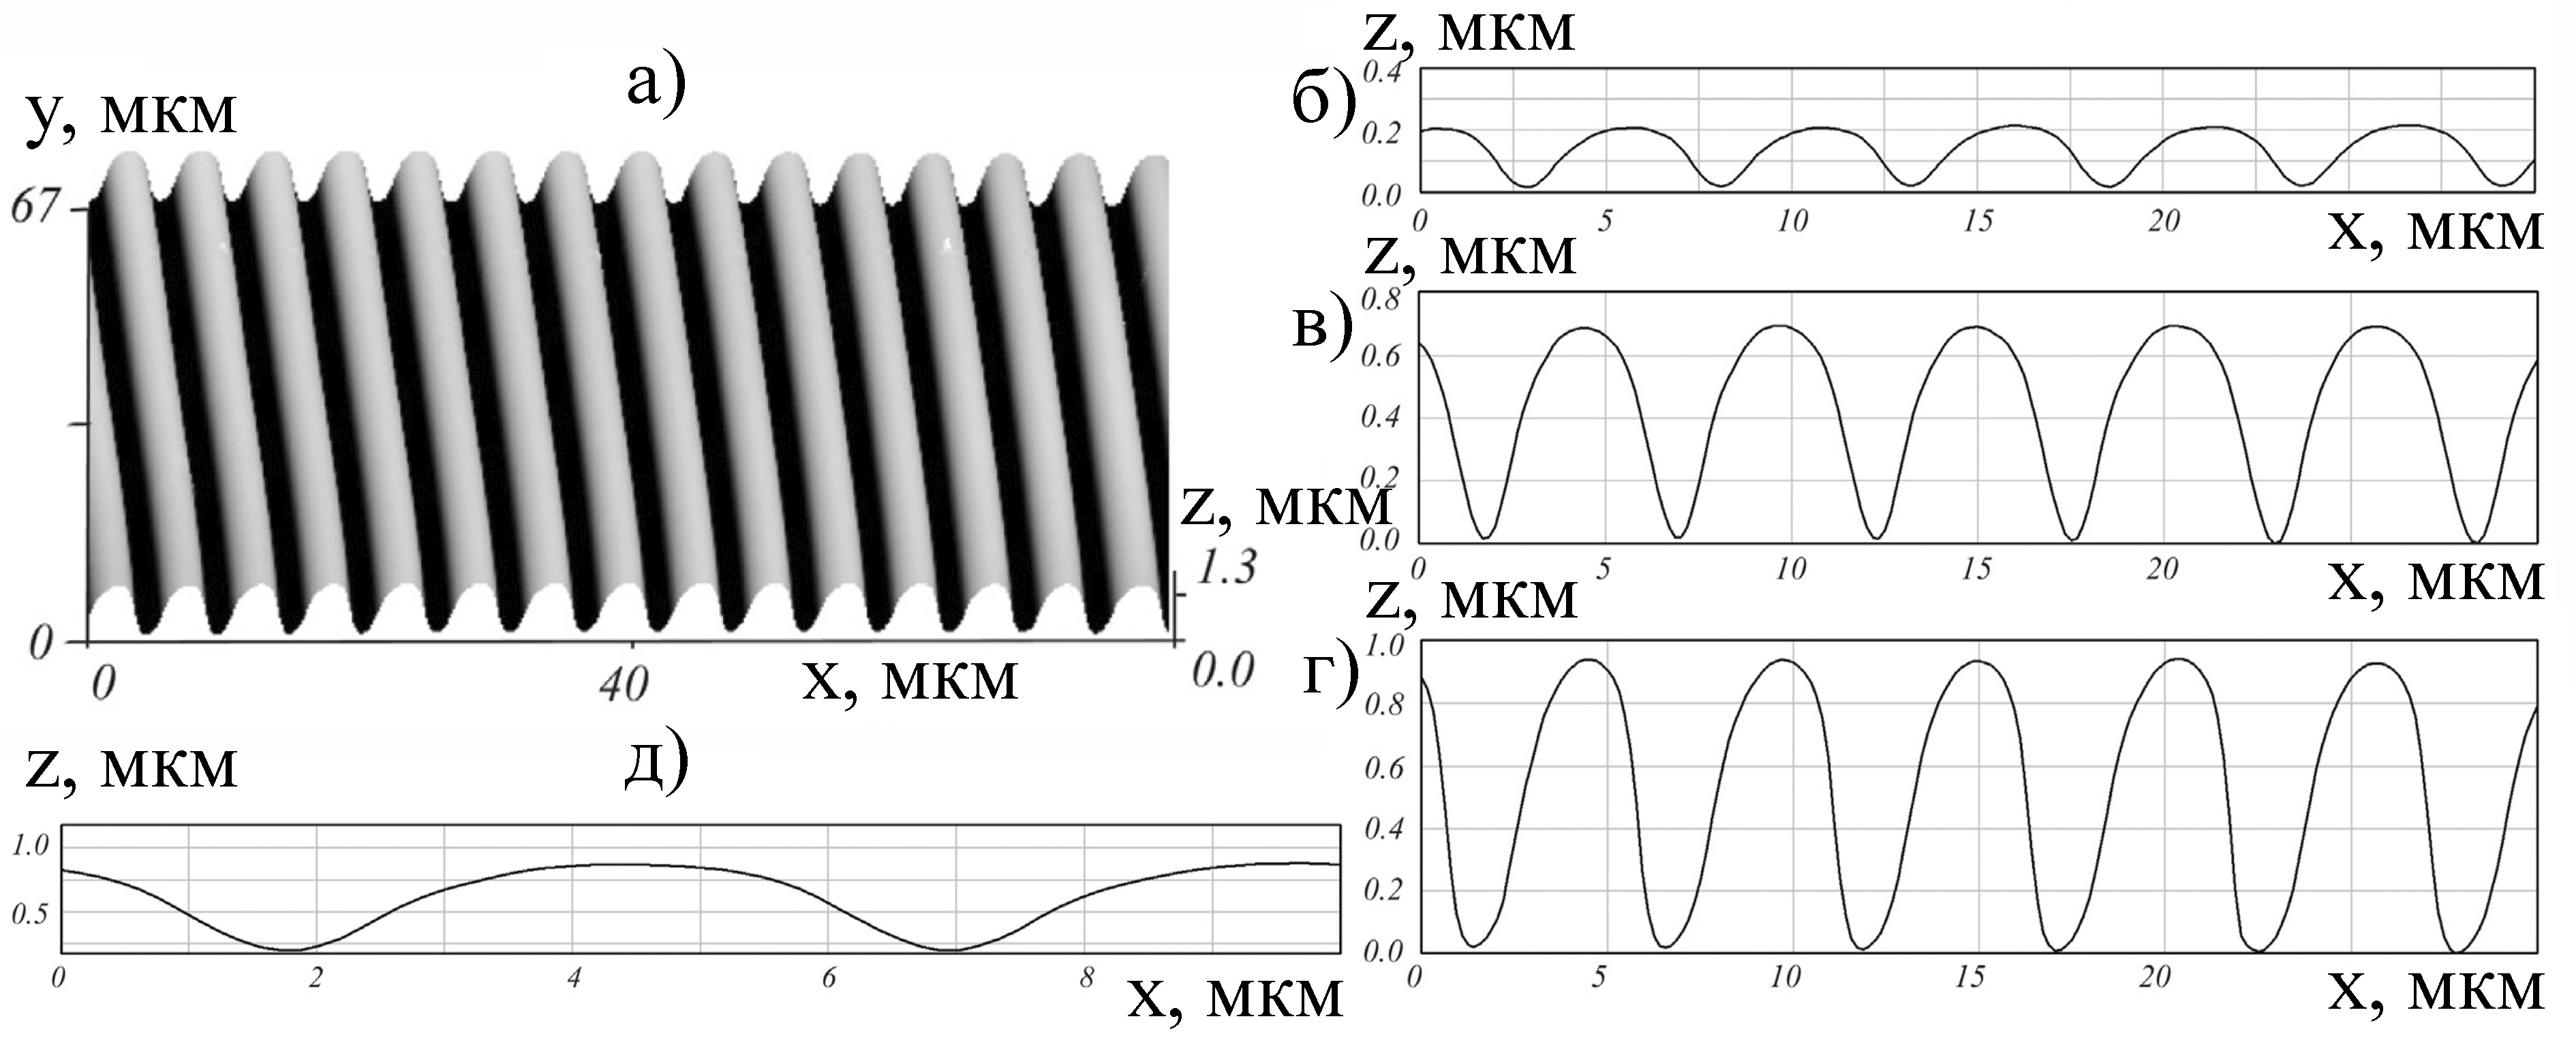
\includegraphics{jpg/DEBER_many_profiles_14pt}
	\caption{Периодические профили, полученные методом СЭЛТР в слое ПММА толщиной 900 нм при экспонировании вдоль серии параллельных линий при температуре 160 $^\circ$C: а) трехмерное изображение; б), в), г) -- профили, полученные при дозах экспонирования 0.05, 0.2 и 0.87 мкКл/см$^2$, соответственно, д) -- изображение профиля в) в масштабе 1:1~\cite{Bruk_2016_mee}.}
	\label{fig:DEBER_many_profiles}
\end{figure}

\begin{figure}[t]
	\centering
	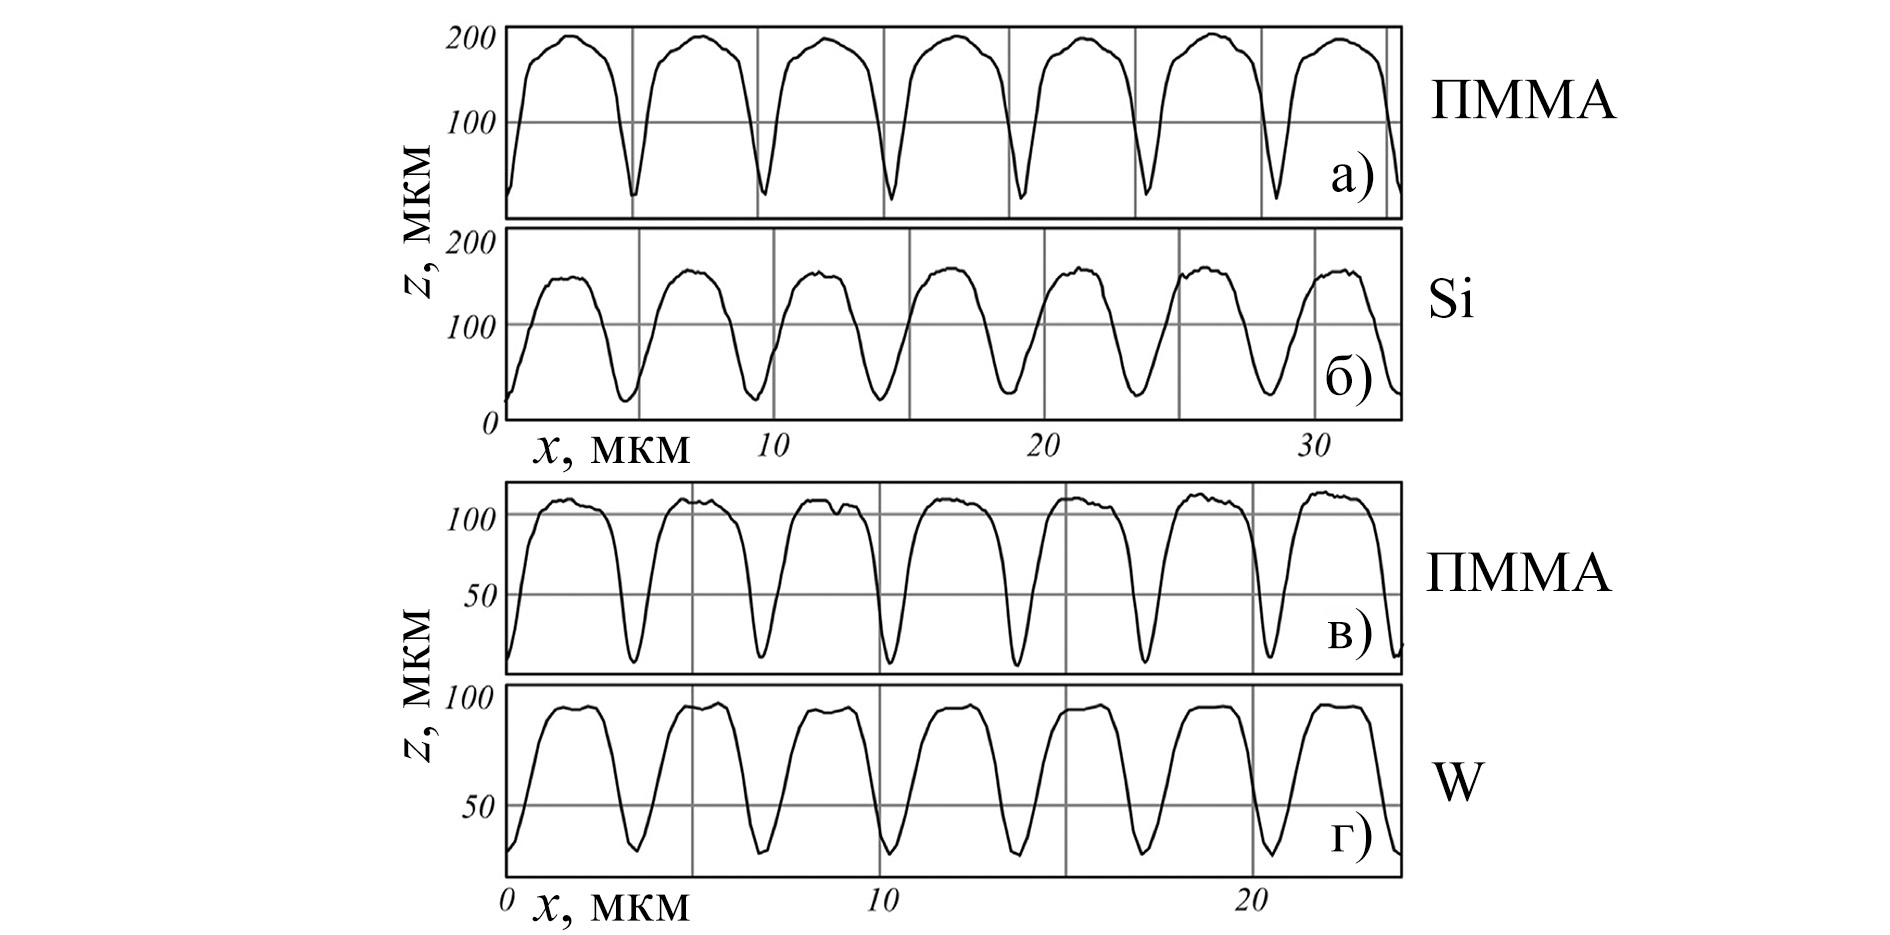
\includegraphics{jpg/DEBER_Si_W_14pt}
	\caption{Сечения профилей до (а) и в)) и после (б) и г)) переноса из ПММА в кремний (Si) и вольфрам (W)~\cite{Bruk_2016_mee}.}
	\label{fig:DEBER_Si_W}
\end{figure}

Для оценки величины латерального разрешения метода СЭЛТР были исследованы профили, полученные при экспонировании резиста остросфокусированным электронным лучом вдоль одиночных линий (рисунок~\ref{fig:DEBER_Ultra}). При диаметре пучка около 10 нм ширина одиночных линий на глубине, равной половине от максимальной глубины травления, составила примерно 200 нм, что было принято за предельное разрешение метода СЭЛТР.

Резюмируя все вышесказанное, можно выделить преимущества и недостатки метода СЭЛТР. К преимуществами данного метода относятся:
\begin{itemize}
	\item высокая производительность метода за счет протекания цепной реакции деполимеризации -- характерные дозы, необходимые для формирования рельефе в резисте методом СЭЛТР в десятки или даже сотни раз меньше, чем характерные дозы в стандартной электронно-лучевой литографии по \textquotedbl мокрой\textquotedbl{} технологии;
	\item простота метода -- формирование дву- и трехмерных структур в резисте происходит за одну вакуумную стадию;
	\item возможность реализации во многих электронно-лучевых системах -- метод СЭЛТР может быть реализован в растровых электронных микроскопах, электронных литографах и др. электронно-лучевых системах с минимальными модификациями (обеспечение возможности нагрева образца и, при необходимости, установка ловушек для мономера);
	\item сглаженный профиль получаемой структуры за счет процессов растекания;
\end{itemize}

В настоящее время главным недостатком метода СЭЛТР, бросающим тень на все его преимущества, является достаточно низкое латеральное разрешение и низкий контраст изображения.

В силу большого количества отдельных процессов, протекающих одновременно в методе СЭЛТР, точный механизм формирования рельефа в резисте является нетривиальным. Экспериментальные методы изучения процесса СЭЛТР, использовавшиеся до настоящего времени, во многом ограничены исследованиями результирующего профиля. В силу своей природы, такой подход не позволяет определить вклад латеральное разрешение метода СЭЛТР отдельных процессов, что существенно затрудняет его оптимизацию. В то же время, при наличии физической модели метода СЭЛТР, определение путей оптимизации метода и границ его применимости стало бы вполне возможным. Построение такой модели могло бы быть основано на выделении основных процессов, определяющих профиль линии в методе СЭЛТР, разработке их физических моделей на основе существующих подходов и дальнейшем объединении в общую модель метода, верифицированную на основе экспериментальных профилей.

\begin{figure}
	\centering
	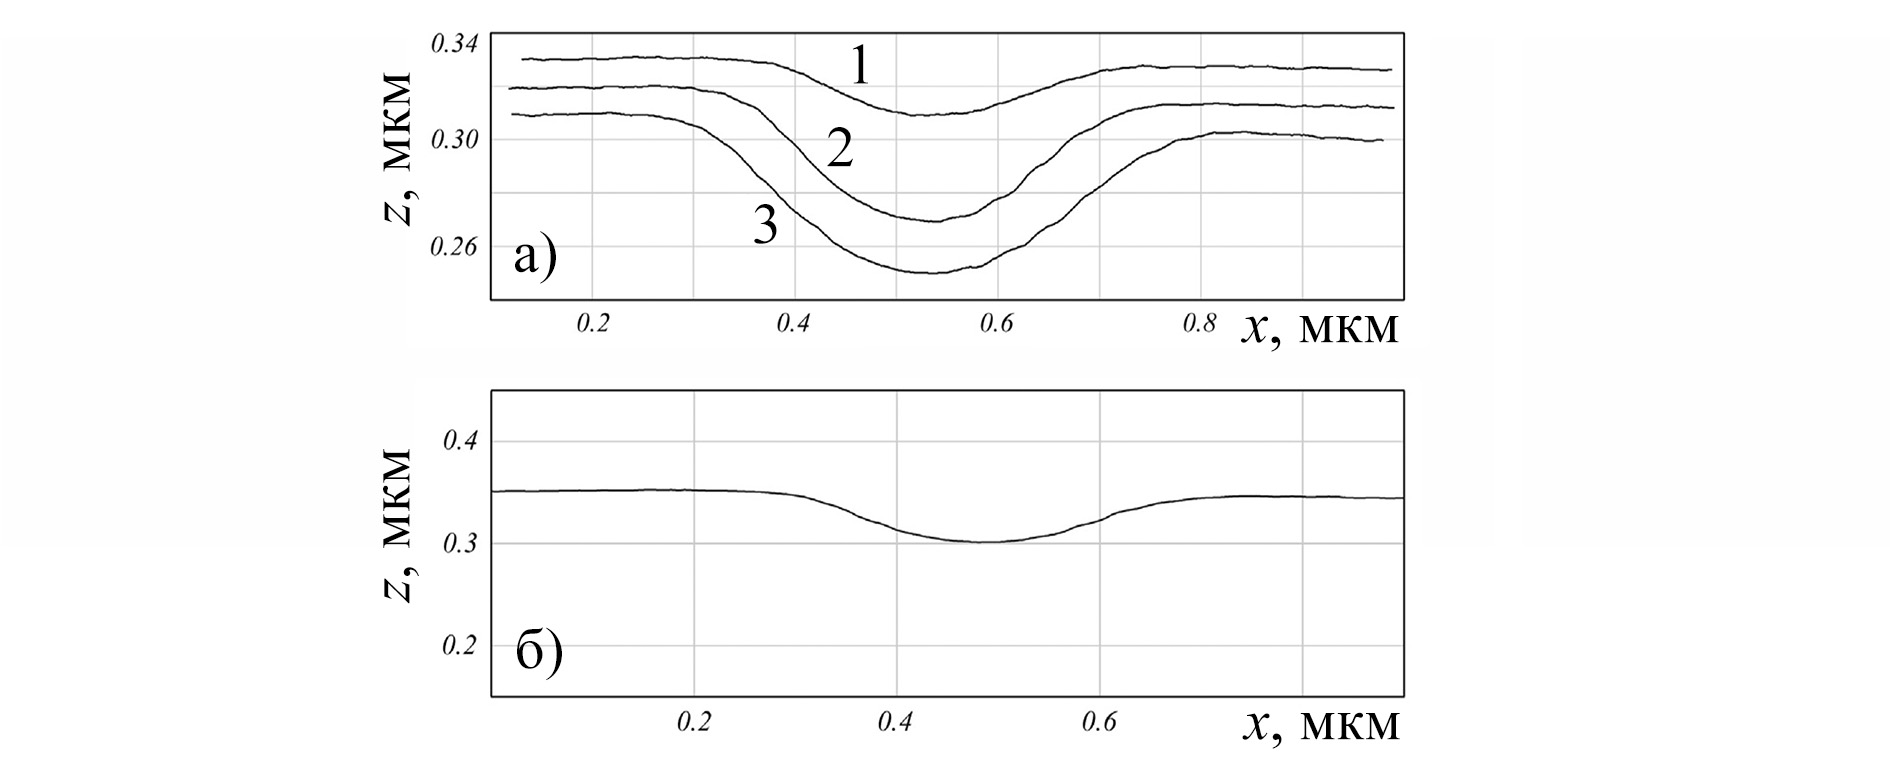
\includegraphics{jpg/DEBER_Ultra_14pt}
	\caption{Профили одиночных линий, полученных в слое ПММА толщиной 80 нм при температуре 116 $^\circ$C при экспонировании остросфокусированным электронным лучом ($\delta \approx$ 10 нм) при времени экспонирования 1 с (а)1), 4 с (а)2) и 16 с (а)3); б) -- изображение профиля а)2 в масштабе 1:1~\cite{Bruk_2016_mee}.}
	\label{fig:DEBER_Ultra}
\end{figure}

Подводя итоги главы, можно выделить несколько важных фактов. Во-первых, в ряде областей востребовано формирование трехмерных микро- и наноструктур, что обеспечивается различными методами, имеющими свои преимущества и недостатки. Во-вторых, исходя из преимуществ и недостатков существующих методов 3D микро- и наноструктурирования, можно заключить, что в настоящее время отсутствует метод, являющийся одновременно высокопроизводительным и простым в реализации. В-третьих, в качестве такого метода может рассматриваться сухое электронно-лучевое травление резиста (СЭЛТР), однако, недостаточное понимание механизма формирования профиля линии в процессе СЭЛТР существенно затрудняет его применение. Таким образом, целесообразным является построение физической модели метода СЭЛТР, что позволит полностью определить возможности данного метода и оптимизировать его параметры для решения различных задач.




